\documentclass[1p]{elsarticle_modified}
%\bibliographystyle{elsarticle-num}

%\usepackage[colorlinks]{hyperref}
%\usepackage{abbrmath_seonhwa} %\Abb, \Ascr, \Acal ,\Abf, \Afrak
\usepackage{amsfonts}
\usepackage{amssymb}
\usepackage{amsmath}
\usepackage{amsthm}
\usepackage{scalefnt}
\usepackage{amsbsy}
\usepackage{kotex}
\usepackage{caption}
\usepackage{subfig}
\usepackage{color}
\usepackage{graphicx}
\usepackage{xcolor} %% white, black, red, green, blue, cyan, magenta, yellow
\usepackage{float}
\usepackage{setspace}
\usepackage{hyperref}

\usepackage{tikz}
\usetikzlibrary{arrows}

\usepackage{multirow}
\usepackage{array} % fixed length table
\usepackage{hhline}

%%%%%%%%%%%%%%%%%%%%%
\makeatletter
\renewcommand*\env@matrix[1][\arraystretch]{%
	\edef\arraystretch{#1}%
	\hskip -\arraycolsep
	\let\@ifnextchar\new@ifnextchar
	\array{*\c@MaxMatrixCols c}}
\makeatother %https://tex.stackexchange.com/questions/14071/how-can-i-increase-the-line-spacing-in-a-matrix
%%%%%%%%%%%%%%%

\usepackage[normalem]{ulem}

\newcommand{\msout}[1]{\ifmmode\text{\sout{\ensuremath{#1}}}\else\sout{#1}\fi}
%SOURCE: \msout is \stkout macro in https://tex.stackexchange.com/questions/20609/strikeout-in-math-mode

\newcommand{\cancel}[1]{
	\ifmmode
	{\color{red}\msout{#1}}
	\else
	{\color{red}\sout{#1}}
	\fi
}

\newcommand{\add}[1]{
	{\color{blue}\uwave{#1}}
}

\newcommand{\replace}[2]{
	\ifmmode
	{\color{red}\msout{#1}}{\color{blue}\uwave{#2}}
	\else
	{\color{red}\sout{#1}}{\color{blue}\uwave{#2}}
	\fi
}

\newcommand{\Sol}{\mathcal{S}} %segment
\newcommand{\D}{D} %diagram
\newcommand{\A}{\mathcal{A}} %arc


%%%%%%%%%%%%%%%%%%%%%%%%%%%%%5 test

\def\sl{\operatorname{\textup{SL}}(2,\Cbb)}
\def\psl{\operatorname{\textup{PSL}}(2,\Cbb)}
\def\quan{\mkern 1mu \triangleright \mkern 1mu}

\theoremstyle{definition}
\newtheorem{thm}{Theorem}[section]
\newtheorem{prop}[thm]{Proposition}
\newtheorem{lem}[thm]{Lemma}
\newtheorem{ques}[thm]{Question}
\newtheorem{cor}[thm]{Corollary}
\newtheorem{defn}[thm]{Definition}
\newtheorem{exam}[thm]{Example}
\newtheorem{rmk}[thm]{Remark}
\newtheorem{alg}[thm]{Algorithm}

\newcommand{\I}{\sqrt{-1}}
\begin{document}

%\begin{frontmatter}
%
%\title{Boundary parabolic representations of knots up to 8 crossings}
%
%%% Group authors per affiliation:
%\author{Yunhi Cho} 
%\address{Department of Mathematics, University of Seoul, Seoul, Korea}
%\ead{yhcho@uos.ac.kr}
%
%
%\author{Seonhwa Kim} %\fnref{s_kim}}
%\address{Center for Geometry and Physics, Institute for Basic Science, Pohang, 37673, Korea}
%\ead{ryeona17@ibs.re.kr}
%
%\author{Hyuk Kim}
%\address{Department of Mathematical Sciences, Seoul National University, Seoul 08826, Korea}
%\ead{hyukkim@snu.ac.kr}
%
%\author{Seokbeom Yoon}
%\address{Department of Mathematical Sciences, Seoul National University, Seoul, 08826,  Korea}
%\ead{sbyoon15@snu.ac.kr}
%
%\begin{abstract}
%We find all boundary parabolic representation of knots up to 8 crossings.
%
%\end{abstract}
%\begin{keyword}
%    \MSC[2010] 57M25 
%\end{keyword}
%
%\end{frontmatter}

%\linenumbers
%\tableofcontents
%
\newcommand\colored[1]{\textcolor{white}{\rule[-0.35ex]{0.8em}{1.4ex}}\kern-0.8em\color{red} #1}%
%\newcommand\colored[1]{\textcolor{white}{ #1}\kern-2.17ex	\textcolor{white}{ #1}\kern-1.81ex	\textcolor{white}{ #1}\kern-2.15ex\color{red}#1	}

{\Large $\underline{12a_{0938}~(K12a_{0938})}$}

\setlength{\tabcolsep}{10pt}
\renewcommand{\arraystretch}{1.6}
\vspace{1cm}\begin{tabular}{m{100pt}>{\centering\arraybackslash}m{274pt}}
\multirow{5}{120pt}{
	\centering
	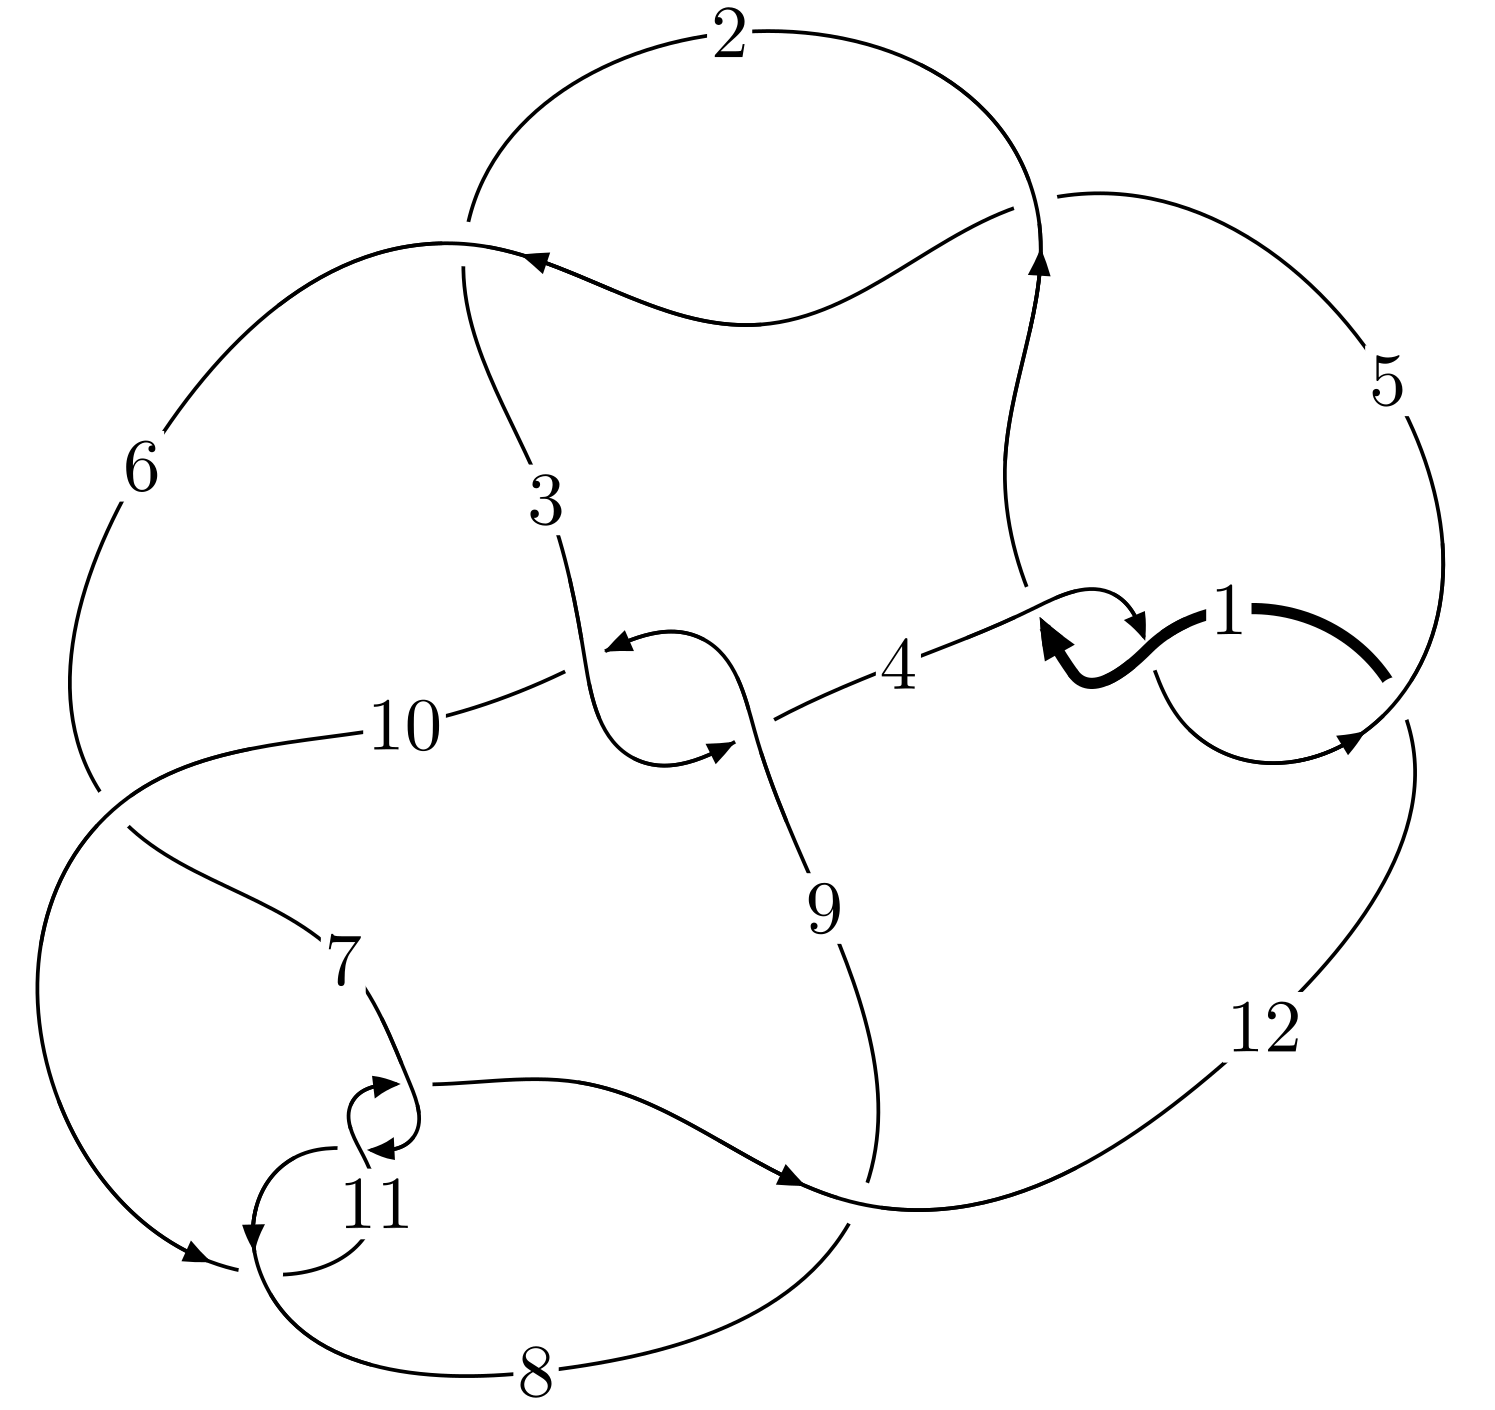
\includegraphics[width=112pt]{../../../GIT/diagram.site/Diagrams/png/1739_12a_0938.png}\\
\ \ \ A knot diagram\footnotemark}&
\allowdisplaybreaks
\textbf{Linearized knot diagam} \\
\cline{2-2}
 &
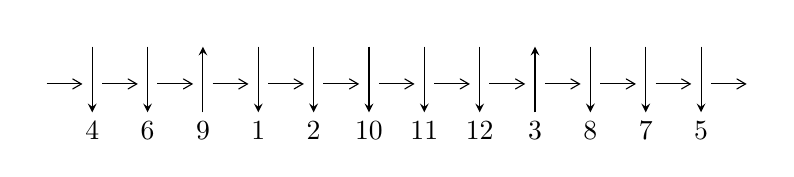
\begin{tikzpicture}[x=20pt, y=17pt]
	% nodes
	\node (C0) at (0, 0) {};
	\node (C1) at (1, 0) {};
	\node (C1U) at (1, +1) {};
	\node (C1D) at (1, -1) {4};

	\node (C2) at (2, 0) {};
	\node (C2U) at (2, +1) {};
	\node (C2D) at (2, -1) {6};

	\node (C3) at (3, 0) {};
	\node (C3U) at (3, +1) {};
	\node (C3D) at (3, -1) {9};

	\node (C4) at (4, 0) {};
	\node (C4U) at (4, +1) {};
	\node (C4D) at (4, -1) {1};

	\node (C5) at (5, 0) {};
	\node (C5U) at (5, +1) {};
	\node (C5D) at (5, -1) {2};

	\node (C6) at (6, 0) {};
	\node (C6U) at (6, +1) {};
	\node (C6D) at (6, -1) {10};

	\node (C7) at (7, 0) {};
	\node (C7U) at (7, +1) {};
	\node (C7D) at (7, -1) {11};

	\node (C8) at (8, 0) {};
	\node (C8U) at (8, +1) {};
	\node (C8D) at (8, -1) {12};

	\node (C9) at (9, 0) {};
	\node (C9U) at (9, +1) {};
	\node (C9D) at (9, -1) {3};

	\node (C10) at (10, 0) {};
	\node (C10U) at (10, +1) {};
	\node (C10D) at (10, -1) {8};

	\node (C11) at (11, 0) {};
	\node (C11U) at (11, +1) {};
	\node (C11D) at (11, -1) {7};

	\node (C12) at (12, 0) {};
	\node (C12U) at (12, +1) {};
	\node (C12D) at (12, -1) {5};
	\node (C13) at (13, 0) {};

	% arrows
	\draw[->,>={angle 60}]
	(C0) edge (C1) (C1) edge (C2) (C2) edge (C3) (C3) edge (C4) (C4) edge (C5) (C5) edge (C6) (C6) edge (C7) (C7) edge (C8) (C8) edge (C9) (C9) edge (C10) (C10) edge (C11) (C11) edge (C12) (C12) edge (C13) ;	\draw[->,>=stealth]
	(C1U) edge (C1D) (C2U) edge (C2D) (C3D) edge (C3U) (C4U) edge (C4D) (C5U) edge (C5D) (C6U) edge (C6D) (C7U) edge (C7D) (C8U) edge (C8D) (C9D) edge (C9U) (C10U) edge (C10D) (C11U) edge (C11D) (C12U) edge (C12D) ;
	\end{tikzpicture} \\
\hhline{~~} \\& 
\textbf{Solving Sequence} \\ \cline{2-2} 
 &
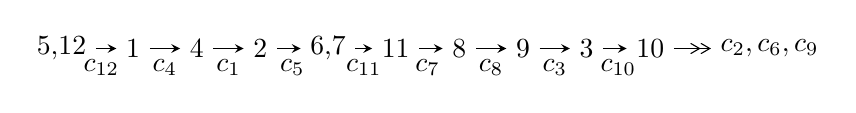
\begin{tikzpicture}[x=23pt, y=7pt]
	% node
	\node (A0) at (-1/8, 0) {5,12};
	\node (A1) at (1, 0) {1};
	\node (A2) at (2, 0) {4};
	\node (A3) at (3, 0) {2};
	\node (A4) at (65/16, 0) {6,7};
	\node (A5) at (41/8, 0) {11};
	\node (A6) at (49/8, 0) {8};
	\node (A7) at (57/8, 0) {9};
	\node (A8) at (65/8, 0) {3};
	\node (A9) at (73/8, 0) {10};
	\node (C1) at (1/2, -1) {$c_{12}$};
	\node (C2) at (3/2, -1) {$c_{4}$};
	\node (C3) at (5/2, -1) {$c_{1}$};
	\node (C4) at (7/2, -1) {$c_{5}$};
	\node (C5) at (37/8, -1) {$c_{11}$};
	\node (C6) at (45/8, -1) {$c_{7}$};
	\node (C7) at (53/8, -1) {$c_{8}$};
	\node (C8) at (61/8, -1) {$c_{3}$};
	\node (C9) at (69/8, -1) {$c_{10}$};
	\node (A10) at (11, 0) {$c_{2},c_{6},c_{9}$};

	% edge
	\draw[->,>=stealth]	
	(A0) edge (A1) (A1) edge (A2) (A2) edge (A3) (A3) edge (A4) (A4) edge (A5) (A5) edge (A6) (A6) edge (A7) (A7) edge (A8) (A8) edge (A9) ;
	\draw[->>,>={angle 60}]	
	(A9) edge (A10);
\end{tikzpicture} \\ 

\end{tabular} \\

\footnotetext{
The image of knot diagram is generated by the software ``\textbf{Draw programme}" developed by Andrew Bartholomew(\url{http://www.layer8.co.uk/maths/draw/index.htm\#Running-draw}), where we modified some parts for our purpose(\url{https://github.com/CATsTAILs/LinksPainter}).
}\phantom \\ \newline 
\centering \textbf{Ideals for irreducible components\footnotemark of $X_{\text{par}}$} 
 
\begin{align*}
I^u_{1}&=\langle 
b- u,\;- u^{12}- u^{11}-5 u^{10}-4 u^9-9 u^8-6 u^7-5 u^6-3 u^5+3 u^4+u^3+3 u^2+a+u,\\
\phantom{I^u_{1}}&\phantom{= \langle  }u^{15}+u^{14}+7 u^{13}+6 u^{12}+19 u^{11}+14 u^{10}+22 u^9+14 u^8+3 u^7+2 u^6-14 u^5-6 u^4-6 u^3-4 u^2+3 u-1\rangle \\
I^u_{2}&=\langle 
u^{59}+2 u^{58}+\cdots+2 b-2,\;u^{59}+3 u^{58}+\cdots+2 a-4,\;u^{60}+3 u^{59}+\cdots-8 u-1\rangle \\
I^u_{3}&=\langle 
b+u,\;a- u+2,\;u^3- u^2+2 u-1\rangle \\
I^u_{4}&=\langle 
- u^2 a- u^2+b- a-1,\;u^2 a+a^2+u^2+2 a+2,\;u^3- u^2+2 u-1\rangle \\
\\
\end{align*}
\raggedright * 4 irreducible components of $\dim_{\mathbb{C}}=0$, with total 84 representations.\\
\footnotetext{All coefficients of polynomials are rational numbers. But the coefficients are sometimes approximated in decimal forms when there is not enough margin.}
\newpage
\renewcommand{\arraystretch}{1}
\centering \section*{I. $I^u_{1}= \langle b- u,\;- u^{12}- u^{11}+\cdots+a+u,\;u^{15}+u^{14}+\cdots+3 u-1 \rangle$}
\flushleft \textbf{(i) Arc colorings}\\
\begin{tabular}{m{7pt} m{180pt} m{7pt} m{180pt} }
\flushright $a_{5}=$&$\begin{pmatrix}0\\u\end{pmatrix}$ \\
\flushright $a_{12}=$&$\begin{pmatrix}1\\0\end{pmatrix}$ \\
\flushright $a_{1}=$&$\begin{pmatrix}1\\u^2\end{pmatrix}$ \\
\flushright $a_{4}=$&$\begin{pmatrix}u\\u^3+u\end{pmatrix}$ \\
\flushright $a_{2}=$&$\begin{pmatrix}u^2+1\\u^4+2 u^2\end{pmatrix}$ \\
\flushright $a_{6}=$&$\begin{pmatrix}- u^5-2 u^3- u\\- u^7-3 u^5-2 u^3+u\end{pmatrix}$ \\
\flushright $a_{7}=$&$\begin{pmatrix}u^{12}+u^{11}+5 u^{10}+4 u^9+9 u^8+6 u^7+5 u^6+3 u^5-3 u^4- u^3-3 u^2- u\\u\end{pmatrix}$ \\
\flushright $a_{11}=$&$\begin{pmatrix}- u^{13}- u^{12}+\cdots+u^2+1\\- u^2\end{pmatrix}$ \\
\flushright $a_{8}=$&$\begin{pmatrix}u^{14}+u^{13}+\cdots-3 u^2-2 u\\u^3+u\end{pmatrix}$ \\
\flushright $a_{9}=$&$\begin{pmatrix}u^{14}+u^{13}+\cdots-3 u^2-3 u\\u^3+u\end{pmatrix}$ \\
\flushright $a_{3}=$&$\begin{pmatrix}- u^8-3 u^6-3 u^4+1\\- u^{10}-4 u^8-5 u^6+3 u^2\end{pmatrix}$ \\
\flushright $a_{10}=$&$\begin{pmatrix}- u^9- u^8-4 u^7-3 u^6-5 u^5-3 u^4- u^2+3 u\\- u^4-2 u^2\end{pmatrix}$\\&\end{tabular}
\flushleft \textbf{(ii) Obstruction class $= -1$}\\~\\
\flushleft \textbf{(iii) Cusp Shapes $= -4 u^{14}-4 u^{13}-26 u^{12}-26 u^{11}-68 u^{10}-66 u^9-78 u^8-74 u^7-16 u^6-16 u^5+38 u^4+34 u^3+16 u^2+24 u-14$}\\~\\
\newpage\renewcommand{\arraystretch}{1}
\flushleft \textbf{(iv) u-Polynomials at the component}\newline \\
\begin{tabular}{m{50pt}|m{274pt}}
Crossings & \hspace{64pt}u-Polynomials at each crossing \\
\hline $$\begin{aligned}c_{1},c_{4},c_{7}\\c_{10},c_{11},c_{12}\end{aligned}$$&$\begin{aligned}
&u^{15}- u^{14}+\cdots+3 u+1
\end{aligned}$\\
\hline $$\begin{aligned}c_{2},c_{5},c_{6}\\c_{8}\end{aligned}$$&$\begin{aligned}
&u^{15}+u^{14}+\cdots+u+1
\end{aligned}$\\
\hline $$\begin{aligned}c_{3},c_{9}\end{aligned}$$&$\begin{aligned}
&u^{15}-7 u^{14}+\cdots+32 u-8
\end{aligned}$\\
\hline
\end{tabular}\\~\\
\newpage\renewcommand{\arraystretch}{1}
\flushleft \textbf{(v) Riley Polynomials at the component}\newline \\
\begin{tabular}{m{50pt}|m{274pt}}
Crossings & \hspace{64pt}Riley Polynomials at each crossing \\
\hline $$\begin{aligned}c_{1},c_{4},c_{7}\\c_{10},c_{11},c_{12}\end{aligned}$$&$\begin{aligned}
&y^{15}+13 y^{14}+\cdots+y-1
\end{aligned}$\\
\hline $$\begin{aligned}c_{2},c_{5},c_{6}\\c_{8}\end{aligned}$$&$\begin{aligned}
&y^{15}-15 y^{14}+\cdots+y-1
\end{aligned}$\\
\hline $$\begin{aligned}c_{3},c_{9}\end{aligned}$$&$\begin{aligned}
&y^{15}+7 y^{14}+\cdots-320 y-64
\end{aligned}$\\
\hline
\end{tabular}\\~\\
\newpage\flushleft \textbf{(vi) Complex Volumes and Cusp Shapes}
$$\begin{array}{c|c|c}  
\text{Solutions to }I^u_{1}& \I (\text{vol} + \sqrt{-1}CS) & \text{Cusp shape}\\
 \hline 
\begin{aligned}
u &= -0.864712 + 0.110290 I \\
a &= -1.86907 - 0.45625 I \\
b &= -0.864712 + 0.110290 I\end{aligned}
 & -11.11480 + 6.35352 I & -15.5001 - 4.2472 I \\ \hline\begin{aligned}
u &= -0.864712 - 0.110290 I \\
a &= -1.86907 + 0.45625 I \\
b &= -0.864712 - 0.110290 I\end{aligned}
 & -11.11480 - 6.35352 I & -15.5001 + 4.2472 I \\ \hline\begin{aligned}
u &= \phantom{-}0.105102 + 1.139200 I \\
a &= -0.439069 + 0.083556 I \\
b &= \phantom{-}0.105102 + 1.139200 I\end{aligned}
 & \phantom{-}4.69451 - 2.19799 I & -5.25826 + 3.25670 I \\ \hline\begin{aligned}
u &= \phantom{-}0.105102 - 1.139200 I \\
a &= -0.439069 - 0.083556 I \\
b &= \phantom{-}0.105102 - 1.139200 I\end{aligned}
 & \phantom{-}4.69451 + 2.19799 I & -5.25826 - 3.25670 I \\ \hline\begin{aligned}
u &= \phantom{-}0.811305\phantom{ +0.000000I} \\
a &= \phantom{-}2.34658\phantom{ +0.000000I} \\
b &= \phantom{-}0.811305\phantom{ +0.000000I}\end{aligned}
 & -6.37976\phantom{ +0.000000I} & -14.9760\phantom{ +0.000000I} \\ \hline\begin{aligned}
u &= -0.423940 + 1.181130 I \\
a &= -1.389210 + 0.220558 I \\
b &= -0.423940 + 1.181130 I\end{aligned}
 & -4.55475 + 2.89595 I & -9.71000 - 3.23135 I \\ \hline\begin{aligned}
u &= -0.423940 - 1.181130 I \\
a &= -1.389210 - 0.220558 I \\
b &= -0.423940 - 1.181130 I\end{aligned}
 & -4.55475 - 2.89595 I & -9.71000 + 3.23135 I \\ \hline\begin{aligned}
u &= \phantom{-}0.360108 + 1.291100 I \\
a &= \phantom{-}2.54683 + 0.20383 I \\
b &= \phantom{-}0.360108 + 1.291100 I\end{aligned}
 & \phantom{-}1.68042 - 8.43141 I & -6.38008 + 6.14293 I \\ \hline\begin{aligned}
u &= \phantom{-}0.360108 - 1.291100 I \\
a &= \phantom{-}2.54683 - 0.20383 I \\
b &= \phantom{-}0.360108 - 1.291100 I\end{aligned}
 & \phantom{-}1.68042 + 8.43141 I & -6.38008 - 6.14293 I \\ \hline\begin{aligned}
u &= \phantom{-}0.035636 + 1.359960 I \\
a &= -0.27580 - 2.64222 I \\
b &= \phantom{-}0.035636 + 1.359960 I\end{aligned}
 & \phantom{-}9.79675 - 2.45365 I & \phantom{-}1.09794 + 3.27080 I\\
 \hline 
 \end{array}$$\newpage$$\begin{array}{c|c|c}  
\text{Solutions to }I^u_{1}& \I (\text{vol} + \sqrt{-1}CS) & \text{Cusp shape}\\
 \hline 
\begin{aligned}
u &= \phantom{-}0.035636 - 1.359960 I \\
a &= -0.27580 + 2.64222 I \\
b &= \phantom{-}0.035636 - 1.359960 I\end{aligned}
 & \phantom{-}9.79675 + 2.45365 I & \phantom{-}1.09794 - 3.27080 I \\ \hline\begin{aligned}
u &= -0.378630 + 1.355350 I \\
a &= -2.48655 - 0.69111 I \\
b &= -0.378630 + 1.355350 I\end{aligned}
 & -1.8779 + 15.2909 I & -7.04558 - 8.68185 I \\ \hline\begin{aligned}
u &= -0.378630 - 1.355350 I \\
a &= -2.48655 + 0.69111 I \\
b &= -0.378630 - 1.355350 I\end{aligned}
 & -1.8779 - 15.2909 I & -7.04558 + 8.68185 I \\ \hline\begin{aligned}
u &= \phantom{-}0.260784 + 0.226947 I \\
a &= -0.260409 - 0.646690 I \\
b &= \phantom{-}0.260784 + 0.226947 I\end{aligned}
 & -0.369166 - 0.786960 I & -8.71574 + 8.77230 I \\ \hline\begin{aligned}
u &= \phantom{-}0.260784 - 0.226947 I \\
a &= -0.260409 + 0.646690 I \\
b &= \phantom{-}0.260784 - 0.226947 I\end{aligned}
 & -0.369166 + 0.786960 I & -8.71574 - 8.77230 I\\
 \hline 
 \end{array}$$\newpage\newpage\renewcommand{\arraystretch}{1}
\centering \section*{II. $I^u_{2}= \langle u^{59}+2 u^{58}+\cdots+2 b-2,\;u^{59}+3 u^{58}+\cdots+2 a-4,\;u^{60}+3 u^{59}+\cdots-8 u-1 \rangle$}
\flushleft \textbf{(i) Arc colorings}\\
\begin{tabular}{m{7pt} m{180pt} m{7pt} m{180pt} }
\flushright $a_{5}=$&$\begin{pmatrix}0\\u\end{pmatrix}$ \\
\flushright $a_{12}=$&$\begin{pmatrix}1\\0\end{pmatrix}$ \\
\flushright $a_{1}=$&$\begin{pmatrix}1\\u^2\end{pmatrix}$ \\
\flushright $a_{4}=$&$\begin{pmatrix}u\\u^3+u\end{pmatrix}$ \\
\flushright $a_{2}=$&$\begin{pmatrix}u^2+1\\u^4+2 u^2\end{pmatrix}$ \\
\flushright $a_{6}=$&$\begin{pmatrix}- u^5-2 u^3- u\\- u^7-3 u^5-2 u^3+u\end{pmatrix}$ \\
\flushright $a_{7}=$&$\begin{pmatrix}-\frac{1}{2} u^{59}-\frac{3}{2} u^{58}+\cdots+\frac{1}{2} u+2\\-\frac{1}{2} u^{59}- u^{58}+\cdots+6 u+1\end{pmatrix}$ \\
\flushright $a_{11}=$&$\begin{pmatrix}4 u^{59}+\frac{21}{2} u^{58}+\cdots-\frac{67}{2} u-\frac{9}{2}\\- u^{59}- u^{58}+\cdots-13 u-\frac{5}{2}\end{pmatrix}$ \\
\flushright $a_{8}=$&$\begin{pmatrix}-\frac{5}{2} u^{59}-8 u^{58}+\cdots+57 u+14\\-\frac{3}{2} u^{59}-4 u^{58}+\cdots+20 u+\frac{9}{2}\end{pmatrix}$ \\
\flushright $a_{9}=$&$\begin{pmatrix}- u^{59}-4 u^{58}+\cdots+37 u+\frac{19}{2}\\-\frac{3}{2} u^{59}-4 u^{58}+\cdots+20 u+\frac{9}{2}\end{pmatrix}$ \\
\flushright $a_{3}=$&$\begin{pmatrix}- u^8-3 u^6-3 u^4+1\\- u^{10}-4 u^8-5 u^6+3 u^2\end{pmatrix}$ \\
\flushright $a_{10}=$&$\begin{pmatrix}6 u^{59}+14 u^{58}+\cdots-66 u-\frac{29}{2}\\\frac{7}{2} u^{59}+9 u^{58}+\cdots-33 u-\frac{13}{2}\end{pmatrix}$\\&\end{tabular}
\flushleft \textbf{(ii) Obstruction class $= -1$}\\~\\
\flushleft \textbf{(iii) Cusp Shapes $= -\frac{21}{2} u^{59}-17 u^{58}+\cdots-3 u-\frac{19}{2}$}\\~\\
\newpage\renewcommand{\arraystretch}{1}
\flushleft \textbf{(iv) u-Polynomials at the component}\newline \\
\begin{tabular}{m{50pt}|m{274pt}}
Crossings & \hspace{64pt}u-Polynomials at each crossing \\
\hline $$\begin{aligned}c_{1},c_{4},c_{7}\\c_{10},c_{11},c_{12}\end{aligned}$$&$\begin{aligned}
&u^{60}-3 u^{59}+\cdots+8 u-1
\end{aligned}$\\
\hline $$\begin{aligned}c_{2},c_{5},c_{6}\\c_{8}\end{aligned}$$&$\begin{aligned}
&u^{60}+3 u^{59}+\cdots+520 u-137
\end{aligned}$\\
\hline $$\begin{aligned}c_{3},c_{9}\end{aligned}$$&$\begin{aligned}
&(u^{30}+3 u^{29}+\cdots-12 u-8)^{2}
\end{aligned}$\\
\hline
\end{tabular}\\~\\
\newpage\renewcommand{\arraystretch}{1}
\flushleft \textbf{(v) Riley Polynomials at the component}\newline \\
\begin{tabular}{m{50pt}|m{274pt}}
Crossings & \hspace{64pt}Riley Polynomials at each crossing \\
\hline $$\begin{aligned}c_{1},c_{4},c_{7}\\c_{10},c_{11},c_{12}\end{aligned}$$&$\begin{aligned}
&y^{60}+49 y^{59}+\cdots-28 y+1
\end{aligned}$\\
\hline $$\begin{aligned}c_{2},c_{5},c_{6}\\c_{8}\end{aligned}$$&$\begin{aligned}
&y^{60}-43 y^{59}+\cdots-297252 y+18769
\end{aligned}$\\
\hline $$\begin{aligned}c_{3},c_{9}\end{aligned}$$&$\begin{aligned}
&(y^{30}+21 y^{29}+\cdots-208 y+64)^{2}
\end{aligned}$\\
\hline
\end{tabular}\\~\\
\newpage\flushleft \textbf{(vi) Complex Volumes and Cusp Shapes}
$$\begin{array}{c|c|c}  
\text{Solutions to }I^u_{2}& \I (\text{vol} + \sqrt{-1}CS) & \text{Cusp shape}\\
 \hline 
\begin{aligned}
u &= -0.866352 + 0.087987 I \\
a &= -0.71052 - 1.48467 I \\
b &= -0.427481 - 1.154580 I\end{aligned}
 & -7.91257 + 1.72426 I & -12.74360 - 0.42116 I \\ \hline\begin{aligned}
u &= -0.866352 - 0.087987 I \\
a &= -0.71052 + 1.48467 I \\
b &= -0.427481 + 1.154580 I\end{aligned}
 & -7.91257 - 1.72426 I & -12.74360 + 0.42116 I \\ \hline\begin{aligned}
u &= -0.859274 + 0.126720 I \\
a &= -2.20772 + 0.88605 I \\
b &= -0.384752 + 1.346570 I\end{aligned}
 & -6.53967 + 10.84120 I & -11.31201 - 6.59674 I \\ \hline\begin{aligned}
u &= -0.859274 - 0.126720 I \\
a &= -2.20772 - 0.88605 I \\
b &= -0.384752 - 1.346570 I\end{aligned}
 & -6.53967 - 10.84120 I & -11.31201 + 6.59674 I \\ \hline\begin{aligned}
u &= \phantom{-}0.811961 + 0.030859 I \\
a &= \phantom{-}1.90730 + 1.95853 I \\
b &= \phantom{-}0.359515 + 1.269110 I\end{aligned}
 & -2.44025 - 4.21285 I & -10.79867 + 3.36820 I \\ \hline\begin{aligned}
u &= \phantom{-}0.811961 - 0.030859 I \\
a &= \phantom{-}1.90730 - 1.95853 I \\
b &= \phantom{-}0.359515 - 1.269110 I\end{aligned}
 & -2.44025 + 4.21285 I & -10.79867 - 3.36820 I \\ \hline\begin{aligned}
u &= -0.812151 + 0.025025 I \\
a &= \phantom{-}1.154180 - 0.235909 I \\
b &= \phantom{-}0.546996 - 0.494154 I\end{aligned}
 & -5.29824 + 1.96304 I & -14.0240 - 3.7195 I \\ \hline\begin{aligned}
u &= -0.812151 - 0.025025 I \\
a &= \phantom{-}1.154180 + 0.235909 I \\
b &= \phantom{-}0.546996 + 0.494154 I\end{aligned}
 & -5.29824 - 1.96304 I & -14.0240 + 3.7195 I \\ \hline\begin{aligned}
u &= -0.426044 + 1.131210 I \\
a &= -0.727875 - 0.277369 I \\
b &= -0.389512 - 1.332390 I\end{aligned}
 & -3.46235 - 6.23114 I & \phantom{-0.000000 } 0 \\ \hline\begin{aligned}
u &= -0.426044 - 1.131210 I \\
a &= -0.727875 + 0.277369 I \\
b &= -0.389512 + 1.332390 I\end{aligned}
 & -3.46235 + 6.23114 I & \phantom{-0.000000 } 0\\
 \hline 
 \end{array}$$\newpage$$\begin{array}{c|c|c}  
\text{Solutions to }I^u_{2}& \I (\text{vol} + \sqrt{-1}CS) & \text{Cusp shape}\\
 \hline 
\begin{aligned}
u &= -0.770784 + 0.061460 I \\
a &= \phantom{-}1.079330 - 0.274511 I \\
b &= \phantom{-}0.14357 - 1.41247 I\end{aligned}
 & \phantom{-}0.79615 + 4.22762 I & -10.05667 - 4.58015 I \\ \hline\begin{aligned}
u &= -0.770784 - 0.061460 I \\
a &= \phantom{-}1.079330 + 0.274511 I \\
b &= \phantom{-}0.14357 + 1.41247 I\end{aligned}
 & \phantom{-}0.79615 - 4.22762 I & -10.05667 + 4.58015 I \\ \hline\begin{aligned}
u &= -0.427481 + 1.154580 I \\
a &= -1.142560 - 0.223262 I \\
b &= -0.866352 - 0.087987 I\end{aligned}
 & -7.91257 - 1.72426 I & \phantom{-0.000000 } 0 \\ \hline\begin{aligned}
u &= -0.427481 - 1.154580 I \\
a &= -1.142560 + 0.223262 I \\
b &= -0.866352 + 0.087987 I\end{aligned}
 & -7.91257 + 1.72426 I & \phantom{-0.000000 } 0 \\ \hline\begin{aligned}
u &= -0.027147 + 1.235000 I \\
a &= \phantom{-}0.583477 + 0.915228 I \\
b &= \phantom{-}0.668715 - 0.159496 I\end{aligned}
 & \phantom{-}2.08860 + 0.78309 I & \phantom{-0.000000 } 0 \\ \hline\begin{aligned}
u &= -0.027147 - 1.235000 I \\
a &= \phantom{-}0.583477 - 0.915228 I \\
b &= \phantom{-}0.668715 + 0.159496 I\end{aligned}
 & \phantom{-}2.08860 - 0.78309 I & \phantom{-0.000000 } 0 \\ \hline\begin{aligned}
u &= \phantom{-}0.522307 + 0.542494 I \\
a &= -1.97898 + 0.17315 I \\
b &= -0.361715 - 1.287380 I\end{aligned}
 & -1.20998 - 6.18837 I & -9.36869 + 6.76347 I \\ \hline\begin{aligned}
u &= \phantom{-}0.522307 - 0.542494 I \\
a &= -1.97898 - 0.17315 I \\
b &= -0.361715 + 1.287380 I\end{aligned}
 & -1.20998 + 6.18837 I & -9.36869 - 6.76347 I \\ \hline\begin{aligned}
u &= \phantom{-}0.546996 + 0.494154 I \\
a &= -1.138140 + 0.625120 I \\
b &= -0.812151 - 0.025025 I\end{aligned}
 & -5.29824 - 1.96304 I & -14.0240 + 3.7195 I \\ \hline\begin{aligned}
u &= \phantom{-}0.546996 - 0.494154 I \\
a &= -1.138140 - 0.625120 I \\
b &= -0.812151 + 0.025025 I\end{aligned}
 & -5.29824 + 1.96304 I & -14.0240 - 3.7195 I\\
 \hline 
 \end{array}$$\newpage$$\begin{array}{c|c|c}  
\text{Solutions to }I^u_{2}& \I (\text{vol} + \sqrt{-1}CS) & \text{Cusp shape}\\
 \hline 
\begin{aligned}
u &= \phantom{-}0.579343 + 0.445290 I \\
a &= -0.104195 + 0.571803 I \\
b &= -0.357093 + 1.248530 I\end{aligned}
 & -1.51678 + 2.24498 I & -10.41829 + 0.03554 I \\ \hline\begin{aligned}
u &= \phantom{-}0.579343 - 0.445290 I \\
a &= -0.104195 - 0.571803 I \\
b &= -0.357093 - 1.248530 I\end{aligned}
 & -1.51678 - 2.24498 I & -10.41829 - 0.03554 I \\ \hline\begin{aligned}
u &= -0.312553 + 1.230880 I \\
a &= -0.243366 - 1.021580 I \\
b &= \phantom{-}0.17696 + 1.40609 I\end{aligned}
 & \phantom{-}4.37363 - 0.32326 I & \phantom{-0.000000 } 0 \\ \hline\begin{aligned}
u &= -0.312553 - 1.230880 I \\
a &= -0.243366 + 1.021580 I \\
b &= \phantom{-}0.17696 - 1.40609 I\end{aligned}
 & \phantom{-}4.37363 + 0.32326 I & \phantom{-0.000000 } 0 \\ \hline\begin{aligned}
u &= -0.058694 + 1.275980 I \\
a &= \phantom{-}2.05305 + 1.65274 I \\
b &= \phantom{-}0.273445 - 1.345740 I\end{aligned}
 & \phantom{-}6.82843 + 4.21576 I & \phantom{-0.000000 } 0 \\ \hline\begin{aligned}
u &= -0.058694 - 1.275980 I \\
a &= \phantom{-}2.05305 - 1.65274 I \\
b &= \phantom{-}0.273445 + 1.345740 I\end{aligned}
 & \phantom{-}6.82843 - 4.21576 I & \phantom{-0.000000 } 0 \\ \hline\begin{aligned}
u &= \phantom{-}0.358239 + 1.242060 I \\
a &= \phantom{-}0.325203 - 1.127520 I \\
b &= \phantom{-}0.358239 - 1.242060 I\end{aligned}
 & \phantom{-}1.29928\phantom{ +0.000000I} & \phantom{-0.000000 } 0 \\ \hline\begin{aligned}
u &= \phantom{-}0.358239 - 1.242060 I \\
a &= \phantom{-}0.325203 + 1.127520 I \\
b &= \phantom{-}0.358239 + 1.242060 I\end{aligned}
 & \phantom{-}1.29928\phantom{ +0.000000I} & \phantom{-0.000000 } 0 \\ \hline\begin{aligned}
u &= \phantom{-}0.088419 + 1.291380 I \\
a &= -0.283489 - 0.576292 I \\
b &= \phantom{-}0.071835 + 0.504277 I\end{aligned}
 & \phantom{-}4.18867 - 2.01435 I & \phantom{-0.000000 } 0 \\ \hline\begin{aligned}
u &= \phantom{-}0.088419 - 1.291380 I \\
a &= -0.283489 + 0.576292 I \\
b &= \phantom{-}0.071835 - 0.504277 I\end{aligned}
 & \phantom{-}4.18867 + 2.01435 I & \phantom{-0.000000 } 0\\
 \hline 
 \end{array}$$\newpage$$\begin{array}{c|c|c}  
\text{Solutions to }I^u_{2}& \I (\text{vol} + \sqrt{-1}CS) & \text{Cusp shape}\\
 \hline 
\begin{aligned}
u &= -0.357093 + 1.248530 I \\
a &= \phantom{-}0.277613 + 0.172882 I \\
b &= \phantom{-}0.579343 + 0.445290 I\end{aligned}
 & -1.51678 + 2.24498 I & \phantom{-0.000000 } 0 \\ \hline\begin{aligned}
u &= -0.357093 - 1.248530 I \\
a &= \phantom{-}0.277613 - 0.172882 I \\
b &= \phantom{-}0.579343 - 0.445290 I\end{aligned}
 & -1.51678 - 2.24498 I & \phantom{-0.000000 } 0 \\ \hline\begin{aligned}
u &= \phantom{-}0.243342 + 1.288680 I \\
a &= -0.821950 + 0.307839 I \\
b &= -0.276488 - 0.137898 I\end{aligned}
 & \phantom{-}2.60325 - 3.14855 I & \phantom{-0.000000 } 0 \\ \hline\begin{aligned}
u &= \phantom{-}0.243342 - 1.288680 I \\
a &= -0.821950 - 0.307839 I \\
b &= -0.276488 + 0.137898 I\end{aligned}
 & \phantom{-}2.60325 + 3.14855 I & \phantom{-0.000000 } 0 \\ \hline\begin{aligned}
u &= \phantom{-}0.668715 + 0.159496 I \\
a &= -1.85649 - 0.59763 I \\
b &= -0.027147 - 1.235000 I\end{aligned}
 & \phantom{-}2.08860 - 0.78309 I & -8.05433 + 0.68374 I \\ \hline\begin{aligned}
u &= \phantom{-}0.668715 - 0.159496 I \\
a &= -1.85649 + 0.59763 I \\
b &= -0.027147 + 1.235000 I\end{aligned}
 & \phantom{-}2.08860 + 0.78309 I & -8.05433 - 0.68374 I \\ \hline\begin{aligned}
u &= \phantom{-}0.359515 + 1.269110 I \\
a &= \phantom{-}1.51041 - 0.74478 I \\
b &= \phantom{-}0.811961 + 0.030859 I\end{aligned}
 & -2.44025 - 4.21285 I & \phantom{-0.000000 } 0 \\ \hline\begin{aligned}
u &= \phantom{-}0.359515 - 1.269110 I \\
a &= \phantom{-}1.51041 + 0.74478 I \\
b &= \phantom{-}0.811961 - 0.030859 I\end{aligned}
 & -2.44025 + 4.21285 I & \phantom{-0.000000 } 0 \\ \hline\begin{aligned}
u &= -0.361715 + 1.287380 I \\
a &= \phantom{-}0.935893 + 0.612906 I \\
b &= \phantom{-}0.522307 - 0.542494 I\end{aligned}
 & -1.20998 + 6.18837 I & \phantom{-0.000000 } 0 \\ \hline\begin{aligned}
u &= -0.361715 - 1.287380 I \\
a &= \phantom{-}0.935893 - 0.612906 I \\
b &= \phantom{-}0.522307 + 0.542494 I\end{aligned}
 & -1.20998 - 6.18837 I & \phantom{-0.000000 } 0\\
 \hline 
 \end{array}$$\newpage$$\begin{array}{c|c|c}  
\text{Solutions to }I^u_{2}& \I (\text{vol} + \sqrt{-1}CS) & \text{Cusp shape}\\
 \hline 
\begin{aligned}
u &= -0.336582 + 1.312290 I \\
a &= \phantom{-}1.70878 + 1.42762 I \\
b &= \phantom{-}0.12149 - 1.42413 I\end{aligned}
 & \phantom{-}5.10162 + 8.23172 I & \phantom{-0.000000 } 0 \\ \hline\begin{aligned}
u &= -0.336582 - 1.312290 I \\
a &= \phantom{-}1.70878 - 1.42762 I \\
b &= \phantom{-}0.12149 + 1.42413 I\end{aligned}
 & \phantom{-}5.10162 - 8.23172 I & \phantom{-0.000000 } 0 \\ \hline\begin{aligned}
u &= \phantom{-}0.628824\phantom{ +0.000000I} \\
a &= -1.09503\phantom{ +0.000000I} \\
b &= -0.227844\phantom{ +0.000000I}\end{aligned}
 & -1.43510\phantom{ +0.000000I} & -5.45290\phantom{ +0.000000I} \\ \hline\begin{aligned}
u &= \phantom{-}0.273445 + 1.345740 I \\
a &= -2.12347 + 1.22513 I \\
b &= -0.058694 - 1.275980 I\end{aligned}
 & \phantom{-}6.82843 - 4.21576 I & \phantom{-0.000000 } 0 \\ \hline\begin{aligned}
u &= \phantom{-}0.273445 - 1.345740 I \\
a &= -2.12347 - 1.22513 I \\
b &= -0.058694 + 1.275980 I\end{aligned}
 & \phantom{-}6.82843 + 4.21576 I & \phantom{-0.000000 } 0 \\ \hline\begin{aligned}
u &= -0.389512 + 1.332390 I \\
a &= \phantom{-}0.361503 - 0.573917 I \\
b &= -0.426044 - 1.131210 I\end{aligned}
 & -3.46235 + 6.23114 I & \phantom{-0.000000 } 0 \\ \hline\begin{aligned}
u &= -0.389512 - 1.332390 I \\
a &= \phantom{-}0.361503 + 0.573917 I \\
b &= -0.426044 + 1.131210 I\end{aligned}
 & -3.46235 - 6.23114 I & \phantom{-0.000000 } 0 \\ \hline\begin{aligned}
u &= -0.384752 + 1.346570 I \\
a &= -1.06494 - 1.02113 I \\
b &= -0.859274 + 0.126720 I\end{aligned}
 & -6.53967 + 10.84120 I & \phantom{-0.000000 } 0 \\ \hline\begin{aligned}
u &= -0.384752 - 1.346570 I \\
a &= -1.06494 + 1.02113 I \\
b &= -0.859274 - 0.126720 I\end{aligned}
 & -6.53967 - 10.84120 I & \phantom{-0.000000 } 0 \\ \hline\begin{aligned}
u &= \phantom{-}0.17696 + 1.40609 I \\
a &= \phantom{-}0.131316 - 0.931855 I \\
b &= -0.312553 + 1.230880 I\end{aligned}
 & \phantom{-}4.37363 - 0.32326 I & \phantom{-0.000000 } 0\\
 \hline 
 \end{array}$$\newpage$$\begin{array}{c|c|c}  
\text{Solutions to }I^u_{2}& \I (\text{vol} + \sqrt{-1}CS) & \text{Cusp shape}\\
 \hline 
\begin{aligned}
u &= \phantom{-}0.17696 - 1.40609 I \\
a &= \phantom{-}0.131316 + 0.931855 I \\
b &= -0.312553 - 1.230880 I\end{aligned}
 & \phantom{-}4.37363 + 0.32326 I & \phantom{-0.000000 } 0 \\ \hline\begin{aligned}
u &= \phantom{-}0.14357 + 1.41247 I \\
a &= -0.252805 + 0.551347 I \\
b &= -0.770784 - 0.061460 I\end{aligned}
 & \phantom{-}0.79615 - 4.22762 I & \phantom{-0.000000 } 0 \\ \hline\begin{aligned}
u &= \phantom{-}0.14357 - 1.41247 I \\
a &= -0.252805 - 0.551347 I \\
b &= -0.770784 + 0.061460 I\end{aligned}
 & \phantom{-}0.79615 + 4.22762 I & \phantom{-0.000000 } 0 \\ \hline\begin{aligned}
u &= \phantom{-}0.12149 + 1.42413 I \\
a &= -1.37385 + 1.60217 I \\
b &= -0.336582 - 1.312290 I\end{aligned}
 & \phantom{-}5.10162 - 8.23172 I & \phantom{-0.000000 } 0 \\ \hline\begin{aligned}
u &= \phantom{-}0.12149 - 1.42413 I \\
a &= -1.37385 - 1.60217 I \\
b &= -0.336582 + 1.312290 I\end{aligned}
 & \phantom{-}5.10162 + 8.23172 I & \phantom{-0.000000 } 0 \\ \hline\begin{aligned}
u &= \phantom{-}0.071835 + 0.504277 I \\
a &= -0.61146 - 1.51320 I \\
b &= \phantom{-}0.088419 + 1.291380 I\end{aligned}
 & \phantom{-}4.18867 - 2.01435 I & -2.24660 + 4.20023 I \\ \hline\begin{aligned}
u &= \phantom{-}0.071835 - 0.504277 I \\
a &= -0.61146 + 1.51320 I \\
b &= \phantom{-}0.088419 - 1.291380 I\end{aligned}
 & \phantom{-}4.18867 + 2.01435 I & -2.24660 - 4.20023 I \\ \hline\begin{aligned}
u &= -0.276488 + 0.137898 I \\
a &= \phantom{-}3.15020 - 1.98893 I \\
b &= \phantom{-}0.243342 - 1.288680 I\end{aligned}
 & \phantom{-}2.60325 + 3.14855 I & -0.03228 - 4.59727 I \\ \hline\begin{aligned}
u &= -0.276488 - 0.137898 I \\
a &= \phantom{-}3.15020 + 1.98893 I \\
b &= \phantom{-}0.243342 + 1.288680 I\end{aligned}
 & \phantom{-}2.60325 - 3.14855 I & -0.03228 + 4.59727 I \\ \hline\begin{aligned}
u &= -0.227844\phantom{ +0.000000I} \\
a &= \phantom{-}3.02215\phantom{ +0.000000I} \\
b &= \phantom{-}0.628824\phantom{ +0.000000I}\end{aligned}
 & -1.43510\phantom{ +0.000000I} & -5.45290\phantom{ +0.000000I}\\
 \hline 
 \end{array}$$\newpage\newpage\renewcommand{\arraystretch}{1}
\centering \section*{III. $I^u_{3}= \langle b+u,\;a- u+2,\;u^3- u^2+2 u-1 \rangle$}
\flushleft \textbf{(i) Arc colorings}\\
\begin{tabular}{m{7pt} m{180pt} m{7pt} m{180pt} }
\flushright $a_{5}=$&$\begin{pmatrix}0\\u\end{pmatrix}$ \\
\flushright $a_{12}=$&$\begin{pmatrix}1\\0\end{pmatrix}$ \\
\flushright $a_{1}=$&$\begin{pmatrix}1\\u^2\end{pmatrix}$ \\
\flushright $a_{4}=$&$\begin{pmatrix}u\\u^2- u+1\end{pmatrix}$ \\
\flushright $a_{2}=$&$\begin{pmatrix}u^2+1\\u^2- u+1\end{pmatrix}$ \\
\flushright $a_{6}=$&$\begin{pmatrix}-1\\0\end{pmatrix}$ \\
\flushright $a_{7}=$&$\begin{pmatrix}u-2\\- u\end{pmatrix}$ \\
\flushright $a_{11}=$&$\begin{pmatrix}u^2-2 u+1\\- u^2\end{pmatrix}$ \\
\flushright $a_{8}=$&$\begin{pmatrix}- u^2-1\\- u^2+u-1\end{pmatrix}$ \\
\flushright $a_{9}=$&$\begin{pmatrix}- u\\- u^2+u-1\end{pmatrix}$ \\
\flushright $a_{3}=$&$\begin{pmatrix}u\\u^2- u+1\end{pmatrix}$ \\
\flushright $a_{10}=$&$\begin{pmatrix}- u\\- u^2+u-1\end{pmatrix}$\\&\end{tabular}
\flushleft \textbf{(ii) Obstruction class $= 1$}\\~\\
\flushleft \textbf{(iii) Cusp Shapes $= -8 u^2+8 u-20$}\\~\\
\newpage\renewcommand{\arraystretch}{1}
\flushleft \textbf{(iv) u-Polynomials at the component}\newline \\
\begin{tabular}{m{50pt}|m{274pt}}
Crossings & \hspace{64pt}u-Polynomials at each crossing \\
\hline $$\begin{aligned}c_{1},c_{7},c_{12}\end{aligned}$$&$\begin{aligned}
&u^3- u^2+2 u-1
\end{aligned}$\\
\hline $$\begin{aligned}c_{2},c_{6},c_{8}\end{aligned}$$&$\begin{aligned}
&u^3+u^2-1
\end{aligned}$\\
\hline $$\begin{aligned}c_{3},c_{9}\end{aligned}$$&$\begin{aligned}
&u^3
\end{aligned}$\\
\hline $$\begin{aligned}c_{4},c_{10},c_{11}\end{aligned}$$&$\begin{aligned}
&u^3+u^2+2 u+1
\end{aligned}$\\
\hline $$\begin{aligned}c_{5}\end{aligned}$$&$\begin{aligned}
&u^3- u^2+1
\end{aligned}$\\
\hline
\end{tabular}\\~\\
\newpage\renewcommand{\arraystretch}{1}
\flushleft \textbf{(v) Riley Polynomials at the component}\newline \\
\begin{tabular}{m{50pt}|m{274pt}}
Crossings & \hspace{64pt}Riley Polynomials at each crossing \\
\hline $$\begin{aligned}c_{1},c_{4},c_{7}\\c_{10},c_{11},c_{12}\end{aligned}$$&$\begin{aligned}
&y^3+3 y^2+2 y-1
\end{aligned}$\\
\hline $$\begin{aligned}c_{2},c_{5},c_{6}\\c_{8}\end{aligned}$$&$\begin{aligned}
&y^3- y^2+2 y-1
\end{aligned}$\\
\hline $$\begin{aligned}c_{3},c_{9}\end{aligned}$$&$\begin{aligned}
&y^3
\end{aligned}$\\
\hline
\end{tabular}\\~\\
\newpage\flushleft \textbf{(vi) Complex Volumes and Cusp Shapes}
$$\begin{array}{c|c|c}  
\text{Solutions to }I^u_{3}& \I (\text{vol} + \sqrt{-1}CS) & \text{Cusp shape}\\
 \hline 
\begin{aligned}
u &= \phantom{-}0.215080 + 1.307140 I \\
a &= -1.78492 + 1.30714 I \\
b &= -0.215080 - 1.307140 I\end{aligned}
 & \phantom{-}6.04826 - 5.65624 I & -4.98049 + 5.95889 I \\ \hline\begin{aligned}
u &= \phantom{-}0.215080 - 1.307140 I \\
a &= -1.78492 - 1.30714 I \\
b &= -0.215080 + 1.307140 I\end{aligned}
 & \phantom{-}6.04826 + 5.65624 I & -4.98049 - 5.95889 I \\ \hline\begin{aligned}
u &= \phantom{-}0.569840\phantom{ +0.000000I} \\
a &= -1.43016\phantom{ +0.000000I} \\
b &= -0.569840\phantom{ +0.000000I}\end{aligned}
 & -2.22691\phantom{ +0.000000I} & -18.0390\phantom{ +0.000000I}\\
 \hline 
 \end{array}$$\newpage\newpage\renewcommand{\arraystretch}{1}
\centering \section*{IV. $I^u_{4}= \langle - u^2 a- u^2+b- a-1,\;u^2 a+a^2+u^2+2 a+2,\;u^3- u^2+2 u-1 \rangle$}
\flushleft \textbf{(i) Arc colorings}\\
\begin{tabular}{m{7pt} m{180pt} m{7pt} m{180pt} }
\flushright $a_{5}=$&$\begin{pmatrix}0\\u\end{pmatrix}$ \\
\flushright $a_{12}=$&$\begin{pmatrix}1\\0\end{pmatrix}$ \\
\flushright $a_{1}=$&$\begin{pmatrix}1\\u^2\end{pmatrix}$ \\
\flushright $a_{4}=$&$\begin{pmatrix}u\\u^2- u+1\end{pmatrix}$ \\
\flushright $a_{2}=$&$\begin{pmatrix}u^2+1\\u^2- u+1\end{pmatrix}$ \\
\flushright $a_{6}=$&$\begin{pmatrix}-1\\0\end{pmatrix}$ \\
\flushright $a_{7}=$&$\begin{pmatrix}a\\u^2 a+u^2+a+1\end{pmatrix}$ \\
\flushright $a_{11}=$&$\begin{pmatrix}u^2 a- a u+2 u^2+2 a- u+4\\a u+u^2+2\end{pmatrix}$ \\
\flushright $a_{8}=$&$\begin{pmatrix}- u^2 a- a\\- u^2 a+a u- a\end{pmatrix}$ \\
\flushright $a_{9}=$&$\begin{pmatrix}- a u\\- u^2 a+a u- a\end{pmatrix}$ \\
\flushright $a_{3}=$&$\begin{pmatrix}u\\u^2- u+1\end{pmatrix}$ \\
\flushright $a_{10}=$&$\begin{pmatrix}- a u\\- u^2 a+a u- a\end{pmatrix}$\\&\end{tabular}
\flushleft \textbf{(ii) Obstruction class $= 1$}\\~\\
\flushleft \textbf{(iii) Cusp Shapes $= -3 u^2 a+5 a u-3 u^2-3 a+3 u-12$}\\~\\
\newpage\renewcommand{\arraystretch}{1}
\flushleft \textbf{(iv) u-Polynomials at the component}\newline \\
\begin{tabular}{m{50pt}|m{274pt}}
Crossings & \hspace{64pt}u-Polynomials at each crossing \\
\hline $$\begin{aligned}c_{1},c_{7},c_{12}\end{aligned}$$&$\begin{aligned}
&(u^3- u^2+2 u-1)^2
\end{aligned}$\\
\hline $$\begin{aligned}c_{2},c_{6},c_{8}\end{aligned}$$&$\begin{aligned}
&(u^3+u^2-1)^2
\end{aligned}$\\
\hline $$\begin{aligned}c_{3},c_{9}\end{aligned}$$&$\begin{aligned}
&u^6
\end{aligned}$\\
\hline $$\begin{aligned}c_{4},c_{10},c_{11}\end{aligned}$$&$\begin{aligned}
&(u^3+u^2+2 u+1)^2
\end{aligned}$\\
\hline $$\begin{aligned}c_{5}\end{aligned}$$&$\begin{aligned}
&(u^3- u^2+1)^2
\end{aligned}$\\
\hline
\end{tabular}\\~\\
\newpage\renewcommand{\arraystretch}{1}
\flushleft \textbf{(v) Riley Polynomials at the component}\newline \\
\begin{tabular}{m{50pt}|m{274pt}}
Crossings & \hspace{64pt}Riley Polynomials at each crossing \\
\hline $$\begin{aligned}c_{1},c_{4},c_{7}\\c_{10},c_{11},c_{12}\end{aligned}$$&$\begin{aligned}
&(y^3+3 y^2+2 y-1)^2
\end{aligned}$\\
\hline $$\begin{aligned}c_{2},c_{5},c_{6}\\c_{8}\end{aligned}$$&$\begin{aligned}
&(y^3- y^2+2 y-1)^2
\end{aligned}$\\
\hline $$\begin{aligned}c_{3},c_{9}\end{aligned}$$&$\begin{aligned}
&y^6
\end{aligned}$\\
\hline
\end{tabular}\\~\\
\newpage\flushleft \textbf{(vi) Complex Volumes and Cusp Shapes}
$$\begin{array}{c|c|c}  
\text{Solutions to }I^u_{4}& \I (\text{vol} + \sqrt{-1}CS) & \text{Cusp shape}\\
 \hline 
\begin{aligned}
u &= \phantom{-}0.215080 + 1.307140 I \\
a &= \phantom{-}0.162359 - 0.986732 I \\
b &= -0.215080 + 1.307140 I\end{aligned}
 & \phantom{-}6.04826\phantom{ +0.000000I} &                  -6
-1.085931 + 0. 10   I\phantom{ +0.000000I} \\ \hline\begin{aligned}
u &= \phantom{-}0.215080 + 1.307140 I \\
a &= -0.500000 + 0.424452 I \\
b &= -0.569840\phantom{ +0.000000I}\end{aligned}
 & \phantom{-}1.91067 - 2.82812 I & -9.95703 + 1.11003 I \\ \hline\begin{aligned}
u &= \phantom{-}0.215080 - 1.307140 I \\
a &= \phantom{-}0.162359 + 0.986732 I \\
b &= -0.215080 - 1.307140 I\end{aligned}
 & \phantom{-}6.04826\phantom{ +0.000000I} &                  -6
-1.085931 + 0. 10   I\phantom{ +0.000000I} \\ \hline\begin{aligned}
u &= \phantom{-}0.215080 - 1.307140 I \\
a &= -0.500000 - 0.424452 I \\
b &= -0.569840\phantom{ +0.000000I}\end{aligned}
 & \phantom{-}1.91067 + 2.82812 I & -9.95703 - 1.11003 I \\ \hline\begin{aligned}
u &= \phantom{-}0.569840\phantom{ +0.000000I} \\
a &= -1.16236 + 0.98673 I \\
b &= -0.215080 + 1.307140 I\end{aligned}
 & \phantom{-}1.91067 + 2.82812 I & -9.95703 - 1.11003 I \\ \hline\begin{aligned}
u &= \phantom{-}0.569840\phantom{ +0.000000I} \\
a &= -1.16236 - 0.98673 I \\
b &= -0.215080 - 1.307140 I\end{aligned}
 & \phantom{-}1.91067 - 2.82812 I & -9.95703 + 1.11003 I\\
 \hline 
 \end{array}$$\newpage
\newpage\renewcommand{\arraystretch}{1}
\centering \section*{ V. u-Polynomials}
\begin{tabular}{m{50pt}|m{274pt}}
Crossings & \hspace{64pt}u-Polynomials at each crossing \\
\hline $$\begin{aligned}c_{1},c_{7},c_{12}\end{aligned}$$&$\begin{aligned}
&((u^3- u^2+2 u-1)^3)(u^{15}- u^{14}+\cdots+3 u+1)(u^{60}-3 u^{59}+\cdots+8 u-1)
\end{aligned}$\\
\hline $$\begin{aligned}c_{2},c_{6},c_{8}\end{aligned}$$&$\begin{aligned}
&((u^3+u^2-1)^3)(u^{15}+u^{14}+\cdots+u+1)(u^{60}+3 u^{59}+\cdots+520 u-137)
\end{aligned}$\\
\hline $$\begin{aligned}c_{3},c_{9}\end{aligned}$$&$\begin{aligned}
&u^9(u^{15}-7 u^{14}+\cdots+32 u-8)(u^{30}+3 u^{29}+\cdots-12 u-8)^{2}
\end{aligned}$\\
\hline $$\begin{aligned}c_{4},c_{10},c_{11}\end{aligned}$$&$\begin{aligned}
&((u^3+u^2+2 u+1)^3)(u^{15}- u^{14}+\cdots+3 u+1)(u^{60}-3 u^{59}+\cdots+8 u-1)
\end{aligned}$\\
\hline $$\begin{aligned}c_{5}\end{aligned}$$&$\begin{aligned}
&((u^3- u^2+1)^3)(u^{15}+u^{14}+\cdots+u+1)(u^{60}+3 u^{59}+\cdots+520 u-137)
\end{aligned}$\\
\hline
\end{tabular}\newpage\renewcommand{\arraystretch}{1}
\centering \section*{ VI. Riley Polynomials}
\begin{tabular}{m{50pt}|m{274pt}}
Crossings & \hspace{64pt}Riley Polynomials at each crossing \\
\hline $$\begin{aligned}c_{1},c_{4},c_{7}\\c_{10},c_{11},c_{12}\end{aligned}$$&$\begin{aligned}
&((y^3+3 y^2+2 y-1)^3)(y^{15}+13 y^{14}+\cdots+y-1)\\
&\cdot(y^{60}+49 y^{59}+\cdots-28 y+1)
\end{aligned}$\\
\hline $$\begin{aligned}c_{2},c_{5},c_{6}\\c_{8}\end{aligned}$$&$\begin{aligned}
&((y^3- y^2+2 y-1)^3)(y^{15}-15 y^{14}+\cdots+y-1)\\
&\cdot(y^{60}-43 y^{59}+\cdots-297252 y+18769)
\end{aligned}$\\
\hline $$\begin{aligned}c_{3},c_{9}\end{aligned}$$&$\begin{aligned}
&y^9(y^{15}+7 y^{14}+\cdots-320 y-64)(y^{30}+21 y^{29}+\cdots-208 y+64)^{2}
\end{aligned}$\\
\hline
\end{tabular}
\vskip 2pc
\end{document}